\documentclass[twocolumn]{IEEEtran}
%\documentclass[onecolumn]{IEEEtran}
\usepackage{graphicx}
\usepackage{caption}
%\usepackage[numbers]{natbib}
%\usepackage[sort,numbers]{natbib}
\usepackage{verbatim}
\usepackage{subcaption}
\usepackage[nocompress]{cite}
\usepackage{amsmath, amsthm, amssymb}
\usepackage{enumerate}
\usepackage{url}
\usepackage{epstopdf}
\newtheorem{theorem}{Theorem}
\newtheorem{lemma}{Lemma}
\newtheorem{definition}{\bf Definition}
\newtheorem{remark}{Remark}
\theoremstyle{definition}
\newtheorem{example}{Example}
\usepackage{extarrows}
\usepackage{amsfonts}
\usepackage{algorithm, algorithmic}
\usepackage{color}
\usepackage{mathrsfs}
\usepackage{multirow}
\usepackage{amsmath}
\usepackage{cases}
\usepackage{hyperref} %������
\hypersetup{hypertex=true,
            colorlinks=true,
            linkcolor=black,
            anchorcolor=blue,
            citecolor=black}
\makeatletter
\newcommand{\ALOOP}[1]{\ALC@it\algorithmicloop\ #1
  \begin{ALC@loop}}
\newcommand{\ENDALOOP}{\end{ALC@loop}\ALC@it\algorithmicendloop}
\renewcommand{\algorithmicrequire}{\textbf{Input:}}
\renewcommand{\algorithmicensure}{\textbf{Output:}}
\newcommand{\algorithmicbreak}{\textbf{break}}
\newcommand{\BREAK}{\STATE \algorithmicbreak}
\makeatother
% *** GRAPHICS RELATED PACKAGES ***
%
\ifCLASSINFOpdf
\else
\fi
\hyphenation{op-tical net-works semi-conduc-tor}

\begin{document}
\title{Robust Power Control and Task Offloading for Cloud Assisted MEC in Vehicular Networks}
\begin{comment}
\author{
\thanks{Zhixin Liu, Sainan Wang
are with the Institute of Electrical Engineering, Yanshan
University, Qinhuangdao 066004, China.
}}
\end{comment}
\markboth{Manuscript}{?}
\maketitle
\begin{abstract}
Cloud-assisted mobile-edge computing (C-MEC) has been witnessed as a novel solution for task offloading in vehicular networks, which is able to provide rich computing resources. In this paper, a robust power control scheme is proposed to offload the computation task and maximize the utility of C-MEC networks. However,
an uncertain channel state seriously affects the stable transmission of the offloading task. The first-order Markov process is adopted to simulate channel uncertainty, where vehicular mobility is considered. Moreover, channel reusing is assumed due to the limited spectrum resources, which leads to complex co-channel interference and communication delay. To depress the above challenges, probability constraints of signal links are constructed to ensure communication quality. A Bernstein approximations method is adopted to transform the original constraints into solvable ones. Scrupulously, the block coordinate descent (BCD) method and the successive convex approximation (SCA) technique are further adopted to solve the nonconvex robust optimization framework. A joint robust power control and task offloading scheduling algorithm is proposed further to approach the optimal solutions. Numerical simulations are performed to evaluate the system performances, and the results indicate that the proposed algorithm is effective and outperform the benchmarks, especially in communication environments with channel uncertainty.
\end{abstract}
\begin{keywords}
Internet of Vehicle (IoV), Robust Power Control, Edge Computing, Computation Offloading,
\end{keywords}
\section{Introduction}\label{introduction}
Mobile-edge computing (MEC) and mobile cloud computing (MCC), as two new architectures for the emerging 5G networks, have been increasingly developing to support task offloading for Internet of Things devices, especially providing the low-latency and high-reliability computing services \cite{sym2019}. At the edge of the network center, MEC can reduce the transmission delay and provide computing resources to the vehicle users to relieve the computing pressures \cite{Wang2020}. However, the computing resources of MEC are still inadequately facing a large number of computing tasks. Considering the rich computing resources provided by cloud computing, cloud-based computing networks have been developed to address the explosive-growth requirements of computation offloading. However, cloud computing centers tend to be far from the road. In the high-dynamic Internet of Vehicles, the data produced by vehicles must be processed in a short period \cite{Pang2021}. Therefore, the C-MEC is expected to solve this problem, a network architecture that has both rich computing resources and reduced transmission latency.

However, for the current Mobile-Edge computing that enable vehicular networks, interference in the dense vehicle scenario often leads to acutely poor communication Quality of Service (QoS). In addition, vehicle mobility leads to an uncertain channel state and further affects the stability of communication. So joint power control and computing resource allocation in the multi-vehicles, multi-MEC system will resolve the task offloading problem in a C-MEC vehicular network and will guarantee the QoS.

However, for the current Mobile-Edge computing that enables vehicular networks, interference in the dense vehicle scenario often leads to acutely poor communication Quality of Service (QoS). In addition, a vehicle��s mobility leads to an uncertain channel state and further affects the stability of communication. So joint power control and computing resource allocation in multi-vehicles, the multi-MEC system will resolve the task offloading problem in a C-MEC vehicular network and will guarantee the QoS.
\subsection{Related Works}
Recently, some works have been devoted to an IoV edge computing network, consisting of a cloud computing layer and MEC layer vehicle network architectures. In \cite{Zhou2019}, a hierarchical computing framework for vehicular networks is proposed which is composed of the control layer, the vehicular edge computing server layer, and the vehicular network layer. Dai et al. investigate the service scenario of cooperative computation offloading in MEC-assisted service architecture, where multiple MEC servers and remote cloud offload computation-intensive tasks in a collaborative way \cite{Dai2022}. Some papers focused on the problem of computation offloading in the C-MEC vehicular network scenario. Tan and Hu designed a joint communication, caching, and computing problem for achieving the operational excellence and cost efficiency of vehicular networks \cite{Tan2018}. Wang et al. \cite{Wang2020} formulated the problem as a generalized NE problem and presented a game theory algorithm to analyze the equilibrium problem. Wang et al. \cite{Wang2022} develop a distributed clustering mechanism designed to classify vehicles into multiple cooperative edge servers and maximize the total revenue in the entire scheduling duration. Li et al. \cite{Li2023} construct an analytical model of the service cache at the edge of the vehicle, mainly considering the computational task offloading and task interdependence between RSUs. In summary, most of the existing works only optimized one of the two indexes power control and computing resource allocation. It is assumed in some research that the vehicles use a constant transmit power while our approach optimizes the vehicle��s transmit power and the computing resource allocation in a multi-vehicles, multi-MEC system considered. In this case, it caused a new problem because the objective function is difficult to handle. Nemirovski and Shapiro have proposed a convex approximation approach that can solve it \cite{Nemirovski2007}. Aiming at the non-convex of the problem with two variables, some research decouples the original problem into two subproblems and deploys the block coordinate descent (BCD) method.

Unlike the traditional mobile communications networks with low mobility, the Doppler effect in the high mobility of vehicles poses a challenge to C-MEC communication, when the fast-moving vehicles communicate with different MEC servers, the deterministic channel state information (CSI) is no longer sufficient to describe the channel state in network scenarios with dynamic characteristics, the generated Doppler effect has a significant influence on the small-scale fading of CSI and thereby causing fast channel variations. In other words, the CSIs used are outdated. The First-order Gauss-Markov process is adopted to describe the impacts of the Doppler frequency shift on the channel in \cite{Liu2019}. Moreover, in order to get the outstanding performance with low communication delay and computing delays, vehicle equipment has a reduced tolerance for delay and transmission reliability, so higher requirements are put forward. Li et al. introduce the outage probability constraint to guarantee the reliability of vehicular links \cite{Li2020}. Considering that the exact expression contains the exponential integral function, to make it tractable, it is necessary to consider an approximate closed-form expression such that the computational complexity can be reduced.

In the C-MEC vehicular networks, authorized vehicles with spectrum resources can directly communicate with the RSU. However, the scarce spectrum resources appear inadequate in high-density vehicular networks \cite{Xie2020}. Zhou et al. investigated dynamic sharing of the 5G spectrum and proposed a sharing architecture of DSRC and the 5G spectrum for immersive experience-driven vehicular communications \cite{Zhou2017}. Tran et al. design a holistic solution for joint task offloading and resource allocation in a multi-server MEC-assisted network \cite{Tran2019}. It can be seen effective channel reusing is crucial when the spectrum resources are scarce \cite{Liang2021}. But this can cause problems with interference, interference caused by channel reuse in the vehicle communication scenario often leads to acutely poor communication quality. Then, to deal with the interference constraint, the probability constraint is constructed to depress the uncertain co-channel interference, and the Bernstein approximation method is used to transform it into a solvable closed form, the method has commonly been used to deal with the difficult handling non-convex problem \cite{Wang2015}. To deal with the outage probability constraint, Xiao et al. assume the CSIs are obtained through channel estimation \cite{Xiao2020}. Therefore, the outage constraint is transformed according to the Bernstein-type inequality to make it a deterministic optimization problem \cite{Chen2022}. The Bernstein method is also used because of the characteristics of constraints in this paper.
\subsection{Contributions}
In this paper, a robust power control and task offloading algorithm is proposed for the cloud assisted MEC in vehicular networks with highly dynamic vehicles. Unlike the existing
unilateral research on power control or computing resources allocation, a highly
collaborative system network is investigated and the communication delay and computing delay are guaranteed by probabilistic constraints, vehicle QoS is also guaranteed in the framework. The main contributions of this paper include the following aspects:

\begin{itemize}

  \item We present a C-MEC vehicular networks for computation offloading architecture. For MEC layer, which has moderate computation capacity and deploys close to networks, can be used to assist the vehicles. Cloud computing layer, can be used to process the large-scale, delay-insensitive data that MEC layer can not process. This network architecture can both reduce transmission time and provide large computing resource.
  \item The first-order Markov process is introduced to resolve the channel uncertainty caused by the high-speed movement of vehicles, built a reasonable and feasible IoV network scenario is constructed to more realistically describe the dynamic characteristics of the Internet of Vehicles. The Bernstein approximation method is improved to deal with non-convex outage constraint in large-scale dynamic vehicle network environments.
  \item We propose an efficient hybrid transmission task scheduling strategy, V2R transmission is adopted to minimize the delay when the task-initiating vehicle cannot complete the task independently under C-MEC vehicular networks, and the BCD method is introduced to solve complex optimization problem.
\end{itemize}

The remainder of this paper is organized as follows: the model of power control and task offloading for cloud assisted MEC in vehicular networks is established defines in Section \ref{System model}. In Section \ref{Problem solutions}, the probability constraints and the objective function are formulated, and then give the problem solutions. In Section \ref{Simulation results and performance analysis}, simulation results and performance analysis are presented. Finally, we draw a conclusion in Section \ref{Conclusions}.
%II��IV��III��V%
\section{System model}\label{System model}
In this work, the C-MEC vehicular network is shown in Fig. \ref{F1}, which is composed of the MEC layer, and the cloud computing layer hierarchical architecture of computation offloading, numerous vehicles divided into multiple geographic zones within the RSU��s coverage underlay a cell, each RSU is equipped with a MEC server to provide computation offloading services to the vehicles. We denote the set of vehicles and MEC servers in the mobile system as $\mathcal{V}=\left\{1,\ 2,..., V\right\}$ and $\mathcal{M}=\left\{1,\ 2,..., M\right\}$, respectively. The high-speed mobile wireless communication link is defined as V2RSU (V2R) link, and the fixed wired connection link is defined as RSU to Cloud (R2C) link. The detailed offloading process is described as follows. Firstly, the vehicles offload request messages by the wireless interface, which includes required communication resources, the task ID and submission time, and the maximum tolerable service times of the task to the cloud. Second, the MEC server makes scheduling according to the received request messages, including the task upload server and task computation server. Finally, after the task is uploaded, the task waits in the computing queue until the server's processor processes it. Furthermore, some notations are given in Table \ref{table:1}.
\begin{remark}
In this article, we consider only simplified cases within one time slot to arrive at a tractable solution. Nevertheless, the proposed solution can be easily extended to the multi-segment scenario by adopting a time division multiple access communication technology. That is, the vehicles in each RSU coverage communicate are divided into different collections. Hence, time resource is divided into multi-frames, and each frame is divided into several time slots. Different vehicles access its time slots when they communicate with the RSU.
\end{remark}
\begin{figure}[H]
\centering
\includegraphics[width=9cm]{figures//model2.eps}
\caption{System model.}
\label{F1}
\end{figure}
\begin{table}[!h]
\caption{Notations}
\centering
{\small\begin{tabular}{ll}
\hline
\hline
\label{table:1}
$\textrm{Pr}\{\cdot\}$ & Probability function. \\
%$\mathbit{E}\left(\mathbit{x}\right)$ & Exponential distribution. \\
$\mathbb{R}^k$         & Set of $k$-dimensional real vectors.\\
$\mathbf{f}$ &  Index set of computing resource $\mathbf{f}$$=$$[f_1,\cdots,f_i,\cdots,f_M]$. \\
$\mathbf{p}$ &   Index set of vehicle's power $\mathbf{p}$$=$$[p_1,\cdots,p_i,\cdots,p_M]$. \\
$\mathcal{M}$  & Index set of vehicles over a time slot $\mathcal{M}$$=$$\{1,2,\cdots,M\}$.\\
$\mathcal{V}$  & Index set of all active vehicles $\mathcal{V}$$=$$\{1,2,\cdots,V\}$.\\
$\textrm{E}\{\cdot\}$ &  Mathematical expectation of a random variable. \\
%$\mathcal{J}$  & Index set of all CHs $\mathcal{J}$$=$$\{1,2,\cdots,N\}$. \\
\hline
\hline
\end{tabular}}
\end{table}

\subsection{Communication Model}
Different from the traditional cellular communication, due to the fast mobility of vehicles, the CSI is hard to be estimated precisely. In particular, RSU can only achieve the accurate knowledge of large-scale fading $L^2$ of vehicular to RSU links while the small-scale fading $h$ is greatly influenced by the fast channel variations caused by the Doppler effect. We assume the CSIs are obtained through channel estimation \cite{Xiao2020}, Therefore, we model the small-scale fading channel estimation of $h$ by using the first-order Gauss-Markov process \cite{Kim2011} in each transmission time interval as follows,
\begin{eqnarray}\label{E1}
h=\xi{\widetilde{h}}+\sqrt{1-\xi^2}\zeta,
\end{eqnarray}
we assume that the estimated channel gain $\widetilde{h}$ denotes the estimate of $h$ and ${\widetilde{h}}^2$ is exponentially distributed with unit mean \cite{Sakr2014}. Furthermore, $\xi\in\left(0,1\right)$ represents the correlation coefficient over V2R link, and $\zeta$ stands for the channel gain and follows a complex Gaussian distribution $\zeta\sim CN\left(0,\delta^2\right)$ and independent and uncorrelated of $\widetilde{h}$. The coefficient $\left(0<\zeta<1\right)$ quantifies the channel correlation between the two consecutive time slots and we assume that time correlation coefficient $\zeta$ is same for all vehicles. According to the Jakes statistical model for the fading channel \cite{Kim2011}, $\zeta$ is given as $\zeta=J_0\left(2\pi f_{max}T_s\right)$, where $J_0$ is the zero-order Bessel function of the first kind. $f_{max}=\bar{\nu}f_c/c $ is the maximum Doppler frequency, where $\bar{\nu}$ indicates the vehicle speed, $f_c$ indicates the carrier frequency at 5.9 Ghz, and $c=3\times{10}^8m/s$, $T_s$ is a period feedback latency, both transmitter vehicles and RSU can know the accurate $\zeta$.

Based on the aforementioned discussion, the mobile V2R channel power gain of the effective links and interference links in $k$th time slot from $i$th transmitter to $j$th receiver can be expressed as a shared expression:
\begin{eqnarray}\label{E2}
G_{i,j}^k={\widetilde{g}}_{i,j}^k+{\hat{g}}_{i,j}^k,
\end{eqnarray}
where ${\widetilde{g}}_{i,j}^k=L_{i,j}^2{\widetilde{h}}_{i,j}^2\xi_{i,j}^2$, $ {\hat{g}}_{i,j}^k=L_{i,j}^2\left(1-\xi_{i,j}^2\right)\zeta_{i,j}^2\ $, and $ {L_{i,j}^k}^2$ denotes the kth time slot large-scale fading effects including shadow-fading and path loss from $i$th transmitter to $j$th receiver on the road section. Moreover, ${\hat{g}}_{i,j}^k$ is an observed value and ${\widetilde{g}}_{i,j}^k$ expresses an exponential random variable with parameter $\frac{1}{{L_{i,j}^k}^2({1-{\zeta_{i,j}^k}^2})}$ which is fellow as \cite{Xie2020}.

To improve the spectrum utilization and realize multi-vehicles joint communication, V2R communications reuse the same uplink channel. In this case, the Signal-to-Interference-plus-Noise Ratio (SINR) of V2R link can be formulated as,
\begin{eqnarray}\label{E3}
\gamma_i\left(\mathbf{p}\right)=\frac{p_ig_{i,j}}{{\sum_{j=1,j\neq i}^{M}{p_jg_{j,i}}+\sigma^2}},
\end{eqnarray}
where $p_j $ denotes the transmit power of the $j$th vehicles, and $\sigma^2$ is the background noise. Therefore, the deterministic equivalent transmission rate of vehicles calculated by Shannon��s theorem is,
\begin{eqnarray}\label{E4}
{R_i\left(\mathbf{p}\right)=\log}_2{\left(1+\frac{p_ig_{i,j}}{\sum_{j=1,j\neq i}^{M}{p_jg_{j,i}}+\sigma^2}\right)},
\end{eqnarray}
 then the transmission time of vehicle $i$ when sending its task input $d_{i,up}$ in the uplink can be calculated as,
\begin{eqnarray}\label{E5}
t_{i,up}=\frac{d_{i,up}}{R_i\left(\mathbf{p}\right)},
\end{eqnarray}

Therefore, the upload time of each V2R link can be formulated as,
\begin{eqnarray}\label{E6}
t_{i,up}=\frac{d_{i,up}}{W{\log}_2{\left(1+\frac{p_ig_{i,j}}{\sum_{j=1,j\neq i}^{M}{p_jg_{j,i}}+\sigma^2}\right)}},
\end{eqnarray}
where $W$ is the bandwidth of the reused channel, and $d_{i,up}$ is the amount of input data including system settings, program codes, and input parameters, which is necessary to transfer the program execution.

Communication delay is another momentous index that influences the performance of vehicular networks. The packets to RSUs must be in the queue before they transmit at the speed of $R_i$. It is accepted that the process of a packet arriving at the $i$th V2R receiver is a Poisson process with parameter $k_i$, and the length of the data packet obeys the exponential distribution of parameter $\tau_i$. The $M/M/1$ queueing based method can guarantees the vehicular communications reliability \cite{Guo2019}, then we adopted the $M/M/1$ model instructions the relationship between the expected delay and transmission rate of the $i$th V2R links can be expressed as,
\begin{eqnarray}\label{E7}
D_i=\frac{1}{{\tau_iR}_i-k_i}.
\end{eqnarray}

\subsection{Vehicle Computing Model}
let $c_{0}$ denote the number of CPU cycles for computing 1-bit of input data at vehicle $i$ \cite{Zhang2017}, that is atomic and cannot be divided into subtasks \cite{Saleem2021}, it can be obtained through carefully profiling of the task execution \cite{Yang2015}. Then we consider that each vehicle $v\in \mathcal{V}$ has one different computation task at a time, denoted as $c_{i,e}$ CPU cycles specifies the workload, i.e. the amount of computation cost to accomplish the task, $c_{i,e}$ can be obtained through $c_{0}*d_{i,up}$ \cite{Shuang2021}. Each task should be offloaded to the MEC server and then transmission to the cloud server. By offloading the computation task to the MEC server, the vehicles would get more computing resources, however, it would consume additional time for sending the task input in the uplink.

The MEC server at each RSU is able to provide computation offloading service to a vehicle at a time slot. The computing resources are quantified by the fixed rate $\bar{f}$, expressed in terms of number of CPU cycles/s. the vehicle $i$th uploads the input data of task to the nearest RSU, the RSU process the small-scale, delay-sensitive data first, then the RSU forward the remaining data to the remote cloud server, the cloud is able to provide computation offloading service to multiple RSU concurrently. The computing resources made available by cloud to be shared among the associating users are quantified by the computational rate $f_i$, it is still expressed in terms of number of CPU cycles/s. Thus, the latency for computing offloading can be written as,
\begin{eqnarray}\label{E8}
t_{i,exe}=\frac{c_{i,e}}{\bar{f}+f_i}.
\end{eqnarray}

\subsection{Problem  Definition}
Given the computing resource allocation $f_i$, the total delay experienced by vehicle $i$ when offloading its task is given by,
\begin{eqnarray}\label{E9}
 t_i=\frac{c_{i,e}}{\bar{f}+f_i}+T_c,
\end{eqnarray}
the transmission latency between RSU and cloud server is defined as $T_c$, usually it is set to a fix value \cite{Xiao2020}, so the relative utility function in task completion time is characterized by,
\begin{eqnarray}\label{E10}
U_{i,exe}=\frac{t_{max}-t_{i,exe}}{t_{max}},
\end{eqnarray}
where $t_{max}$ is the maximum tolerable threshold of the task completion time, if a task can be completed ahead of deadline $ t_{max}$, the vehicle can get a higher utility, otherwise, it will produce the corresponding loss. Therefore, we define the offloading utility of vehicle $i$ as,
\begin{eqnarray}\label{E11}
\frac{U_{i,exe}}{t_{i,up}},
\end{eqnarray}
denote offloading time cost utilities at a unit.

The joint power control and task offloading will be formulated as an optimization problem in this section, and the goal is to obtain the minimum total system cost composed of latency and transmission rate for all vehicles in the networks. For a given uplink power allocation vector $\mathbf{p}$, and computing resource allocation vector $\mathbf{f}$, we define the system utility as the weighted-sum of all the vehicles�� offloading utilities,
\begin{eqnarray}\label{E12}
U=\sum_{i=1}^{M}\frac{U_{i,exe}}{t_{i,up}}.
\end{eqnarray}

This utility means getting a more enormous execution time utility with a minor upload time cost. We now formulate the Power Control and Task Offloading Problem as a system utility maximization problem, i.e. the robust optimization problem is formulated as follows:
\begin{subequations}
\begin{align}\label{E13a}
%&\  \textbf{P}:U=\max\sum_{i=1}^{M}\frac{U_{i,exe}}{t_{i,up}} &
&\ \max\limits_{\mathbf{p},\mathbf{f}}\emph{U}(\mathbf{p},\mathbf{f})=\max\sum_{i=1}^{M}\frac{U_{i,exe}}{t_{i,up}}&
\end{align}
	\!\!\!\begin{numcases}{s.t.}\label{E13b}
	\!\!\!\textrm{Pr}\left\{\gamma_i\geq\gamma_{th}\right\}\geq1-\varepsilon_1,\\ \label{E13c}
    \!\!\!\textrm{Pr}\left\{\frac{1}{\tau_iR_i-k_i}+\frac{c_{i,e}}{\bar{f}+f_i}\le D_{max}\right\}\geq1-\varepsilon_2,\\  \label{E13d}
	\!\!\!\sum_{i=1}^{N}f_i\le f_{total},\\  \label{E13e}
    \!\!\!0\le p_i\le p_{max}  \label{E13f}
	\end{numcases}
	\label{eq}
\end{subequations}
Where $U$ denotes the network utility, the constraints in the formulation above can be explained as follows: Constraints \eqref{E13b} is used to guarantee the QoS requirements of vehicles, however, due to Large amount of computation caused by time varying network topologies, the real-time SINR is hard to obtain in vehicular communication scenario, and it can be replaced with the long-term SINR since the CSI feedback time interval is very small. $\gamma_i$ denotes the average SINR of the $i$th V2R link when a small CSI feedback time interval is used, in order to ensure that the task is successfully offloaded to the RSU, the SINR should be guaranteed to be no less than the SINR threshold \cite{liu2021}. $\gamma_{th}$ is the SINR threshold for successful detecting the V2R communication. $\textrm{Pr}\left\{\cdot\right\}$ defines the probability of the input. In this case, we introduce the outage probability constraint \eqref{E13b} to guarantee the reliability of vehicular links \cite{Li2020}. $D_{max}$ is the delay bound of the $i$th V2R link in the process of data transmission. $\varepsilon_1$, $ \varepsilon_2 $ are the outage probability thresholds of SINR and delay constraint respectively, where $\varepsilon_1,\varepsilon_2\in\left(0,1\right)$. Constraints \eqref{E13d} state that each MEC server must allocate a positive computing resource to each user associated with it and that the total computing resources allocated to all the associated users must not excess the server��s computing capacity, in another word, the number of applications served by a particular edge cloud should be within its capacity. \eqref{E13c} denote the total latency of communication and computing should be guaranteed to be no less than the time threshold, $p_{max}$ is the maximum transmit power of the transmit vehicle in vehicle communication network, and the transmit power is greater than zero in \eqref{E13e}.
\section{Problem solutions}\label{Problem solutions}
In this section, we proposed a BCD-based algorithm to solve the problem \eqref{E13a}. The BCD method enables the complex original problem to be decomposed into a succession of simpler subproblems \cite{Bertsekas1999}. Motivated by this fact, all variables are divided into two blocks and optimized alternatively.

By fixing the vector $\mathbf{f}$, the problem \eqref{E13a} can be transformed into the following problem.
\begin{subequations}
\begin{align} \label{E14a}
&\  \textbf{P1}:U=\max\sum_{i=1}^{M}\frac{U_{i,exe}}{t_{i,up}} &
\end{align}
	\begin{numcases}{s.t.} \label{E14b}
	\!\!\!\textrm{Pr}\left\{\gamma_i\geq\gamma_{th}\right\}\geq1-\varepsilon_1 \\ \label{E14c}
   \!\!\! \textrm{Pr}\left\{\frac{1}{\tau_iR_i-k_i}+\frac{c_{i,e}}{\bar{f}+f_i}\le
    D_{max}\right\}\geq1-\varepsilon_2\\ \label{E14d}
   \!\!\! 0\le p_i\le p_{max}
	\end{numcases}
	\label{eq}
\end{subequations}
\subsection{Successive Convex Approximation of the Objective Function}
Since the problem \eqref{E14a} is a non-convex and NP-hard because the objective function is a logarithmic form, here, the method of SCA is adopted to relax the problem \eqref{E14a} and make it solvable. Then the nether constraint is introduced to approximate the original function as follows,
\begin{eqnarray}\label{E15}
\begin{array}{ll}
\alpha \ln{\left(z\right)}+\beta\le \ln{\left(1+z\right)},\\
\end{array}
\end{eqnarray}
\begin{comment}
\begin{eqnarray}\label{E6}
\begin{array}{ll}
\alpha \ln{\left(z\right)}+\beta\le \ln{\left(1+z\right)}\\
\left\{
\begin{array}{ll} \hfill
&\alpha=\frac{z_0}{1+z_0}\\
&\beta=\ln{\left(1+z_0\right)}-\frac{z_0}{1+z_0}\ln{\left(z_0\right)}
\end{array}
\right.
\end{array}
\end{eqnarray}
\end{comment}
where $\alpha=\frac{z_0}{1+z_0}$ and $\beta=\ln{\left(1+z_0\right)}-\frac{z_0}{1+z_0}\ln{\left(z_0\right)}$, each term of \eqref{E15} can be represented by $A_k\ln\left(\gamma_k\left(e^{\widetilde{\mathbf{p}}}\right)\right)+B_k$ through successive convex approximation, where $A_k$ and $B_k$ can be chosen as $A_k=\gamma_i/\left(1+\gamma_i\right)$, $B_k=\ln{\left(1+\gamma_i\right)}-A_k\ln{\left(\gamma_i\right)}$, $A_k$=1, $B_k$=0 and each term of objective function can be written as follows,
\begin{eqnarray}\label{E16}
\frac{1}{\ln{2}}\sum_{i=1}^{M}{\frac{U_{i,exe}}{d_{i,up}}\left.\left[{A_k\ln{\left(\gamma\left(p\right)\right)}+B}_k\right.\right]},
\end{eqnarray}
it is still hard to directly calculation because of fractional from of SINR, we use variable substitution, i.e. ${\hat{p}}_i=\ln{p_i}$, $p_i=e^{{\hat{p}}_i}$, then ${\hat{p}}_i\le \ln{p_{max}},\ \forall\ \ 1\le i\le M$
\begin{eqnarray}\label{E17}
U=\max\frac{1}{\ln{2}}\sum_{i=1}^{M}\left.\frac{U_{i,exe}}{d_{i,up}}\left[{A_k\ln{\left(\gamma\left(e^{\widetilde{P}}\right)\right)}+B}_k\right.\right].
\end{eqnarray}

\subsection{Approximate of the Outage Probability Constraint}
It is obvious that the constraint \eqref{E14b} is uncertain and the objective function is a non-convex problem in \eqref{E14a}, so the objective function and constraints are difficult to deal with when determining the optimal solutions. It is necessary to design an algorithm with lower complexity to solve the problem. In this paper, for the uncertain channel gain, considering the fast fading, the statistical constraints is adopted to describe the uncertainty mentioned in the \eqref{E14b}. To pursue a simple form of \eqref{E14b}, a matrix form is introduced, the general form the channel gain is described as,
\begin{eqnarray}\label{E18}
%\textrm{Pr}\left\{\left(G_m\right)^Te^{\widetilde{p}}+\sigma^2\le0\right\}\geq1-\varepsilon_1
\textrm{Pr}\left\{\left(\textbf{G}_m\right)^Te^{\widetilde{p}}+\sigma^2\le0\right\}\geq1-\varepsilon_1,
\end{eqnarray}
where $\textbf{G}_m=\left[G_{1,m},G_{2,m},\ldots,-\frac{G_{m,m}}{\gamma_{th}},\ldots,G_{M,m}\right]^T
$. Furthermore, the Bernstein method is adopted to approximate the probability constraint with channel uncertainty
\begin{theorem}
The outage probability of all cochannel V2R links $ \textrm{Pr}\left\{\gamma_i\geq\gamma_{th}\right\}\geq1-\varepsilon_1$
is reformulated as the separable constraints,
\begin{eqnarray}\label{E19}
\!\!\!\!\!\!\sigma^2+\sum_{i\neq j}^{M}{\chi_{i,j}e^{{\widetilde{p}}_i}}+\sqrt{2\ln\left(\frac{1}{\varepsilon_1}\right)}\left(\sum_{i\neq j}^{M}\left(\sigma_{i,j}\beta_{i,j}p_i\right)^2\right)^\frac{1}{2}\le0,
\end{eqnarray}
where $\chi_{i,j}=\mu_{i,j}^+\alpha_{i,j}+\beta_{i,j}+g_{i,j}$, these parameters (i.e. $\sigma_{i,j}$ and $\alpha_{i,j}$) are deduced to be positive in \cite{Liu2019}. Suppose that the truncated distributions of $G_{i,j}$ have bounded supports $\left[{\widetilde{g}}_{i,j}^k+\alpha_{i,j},{\widetilde{g}}_{i,j}^k+\beta_{i,j}\right]$, ${\widetilde{g}}_{i,j}^k$ is an estimate of $G_{i,j}$, then introduce constants $\alpha_{i,j}=\frac{1}{2}\left(b_{i,j}-a_{i,j}\right)$, $\beta_{i,j}=\frac{1}{2}\left(b_{i,j}+a_{i,j}\right)$ to normalize the supports to $\left[-1,1\right]$ as follows,
\begin{eqnarray}\label{E20}
\xi_{i,j}=\frac{G_{i,j}-{\widetilde{g}}_{i,j}^k-\beta_{i,j}}{\alpha_{i,j}}\in\left[-1,1\right],
\end{eqnarray}
\end{theorem}
in the last term of \eqref{E19}, the variables $p$ are coupled nonlinearly. Hence, directly finding an acceptably good solution to \eqref{E14b} by the Bernstein method is time consuming when the $k$ increases and the number of vehicles is large. Therefore, it is necessary to introduced a $\ell_2$-norm approximate problem for any $\mathbf{x}\in \mathbb{R}^k$. Hence, the last term in \eqref{E19} containing $\ell_2$-norm of the vector $\mathbf{x}=\left[\sigma_{i,1}\beta_{i,1}p_i,\cdots,\sigma_{i,M}\beta_{i,M}p_i\right]$ is further approximated by $\parallel x\parallel_2 \le \parallel x\parallel_1$. Based on these, the constraint in \eqref{E14a} is further formulated as fellow with lower complexity and higher reliability,
\begin{eqnarray}\label{E21}
\sigma^2+\sum_{i\neq j}^{M}{\chi_{i,j}e^{{\widetilde{p}}_i}}+\sqrt{2\ln\left(\frac{1}{\varepsilon_1}\right)}\sum_{i\neq j}^{M}{\left|\sigma_{i,j}\beta_{i,j}\right|e^{{\widetilde{p}}_i}}\le0,
\end{eqnarray}
to pursue a simple form of \eqref{E21}, we define
\begin{eqnarray}\label{E22}
\ \mathrm{\Pi}_i=\sigma^2+\sqrt{2\ln\left(\frac{1}{\varepsilon_1}\right)}\sum_{i\neq j}^{M}{\left|\sigma_{i,j}\beta_{i,j}\right|e^{{\widetilde{p}}_i}}.
\end{eqnarray}

The constraint \eqref{E14c} can be handled by an Integral transformation method. According to constraint \eqref{E14c}, where $D_{max}=D_1+D_2 $, $D_1=\frac{1}{\tau_iR_i-k_i} $, $ D_2=\frac{c_{i,e}}{f_i} $, $ X={\widetilde{h}}^2$ is an exponential random variable with unit mean, i.e. $X\sim e x p{\left(1\right)}$, we can get the feasible power region of the communication delay probability as follows,
\begin{eqnarray}\label{E23}
\left.\left[\ln\left(1-\varepsilon_2\right)-{\hat{g}}_{i,j}^k\right.\right]e^{{\widetilde{p}}_i}+D^\ast\ \le0,
\end{eqnarray}
the proof of the feasible region can be found as follow,
\begin{proof}
The probability constraint of \eqref{E14c} can be transformed to the deterministic one according to the following inference
\begin{equation}\label{E24}
\begin{array}{ll}
\textrm{Pr}\left\{\frac{1}{\tau_iR_i-k_i}+\frac{c_{i,e}}{f_i}\le D_{max}\right\}\\
=\textrm{Pr}\left\{R_i\geq\frac{1}{R_i\left(D_{max}-D_2\right)}+\frac{k_i}{\tau_i}\right\}\\
\!\le1\!-\!\textrm{Pr}\left\{p_i{\widetilde{g}}_{i,j}^k\le\left(I_{th}+\sigma^2\right)2^\frac{1+k_i\left(D_{max}-D_2\right)}{\tau_i\left(D_{max}-D_2\right)}-p_i{\hat{g}}_{i,j}^k\right\}\\
=\!1\!-\!\int_{0}^{\left(I_{th}+\sigma^2\right)2^\frac{1+k_i\left(D_{max}-D_2\right)}{\tau_i\left(D_{max}-D_2\right)}-p_i{\hat{g}}_{i,j}^k}{e^{-x}dx}\!\geq\!1-\varepsilon_2.
\end{array}
\end{equation}

Then, we have the equivalent result of the inequality function in \eqref{E24} as,
\begin{eqnarray}\label{E25}
\left.\left[\ln\left(1-\varepsilon_2\right)-{\hat{g}}_{i,j}^k\right.\right]e^{{\widetilde{p}}_i}+D^\ast\ \le0,
\end{eqnarray}
where $D^\ast=\left(I_{th}+\sigma^2\right)2^\frac{1+k_i\left(D_{max}-D_2\right)}{\tau_i\left(D_{max}-D_2\right)}.$
\end{proof}
In summary, we can obtain a deterministic optimization problem of robust power allocation by transforming the objective function, outage probability constraints, delay constraints, it is expressed as,
\begin{subequations}
\begin{align}\label{E26}
&\ \!\!\!\textbf{P1}:\max\limits_{\mathbf{p}}\frac{1}{\ln{2}}\sum_{i=1}^{M}\left.\frac{U_{i,exe}}{d_{i,up}}\left[{A_k\ln{\left(\gamma\left(e^{\widetilde{P}}\right)\right)}+B}_k\!\!\right.\right] &
%\max\limits_{\mathbf{p},\mathbf{f}}\emph{U}(\mathbf{p},\mathbf{f})    (\mathbf{p})
%\!\!\!\textbf{P1}:\max\frac{1}{\ln{2}}\sum_{i=1}^{M}\left.\frac{U_{i,exe}}{d_{i,up}}\left[{A_k\ln{\left(\gamma\left(e^{\widetilde{P}}\right)\right)}+B}_k\right.\right]
\end{align}
\begin{numcases}{s.t.}
	\sum_{i=1}^{M}{\chi_{i,j}e^{{\widetilde{p}}_i}}+\mathrm{\Pi}_i\le0\\
   \left.\left[\ln\left(1-\varepsilon_2\right)-{\hat{g}}_{i,j}^k\right.\right]e^{{\widetilde{p}}_i}+D^\ast\le0\\
   -\infty\le{\widetilde{p}}_i\le \ln{p_{i,max}}
	\end{numcases}
	%\label{eq}
\end{subequations}

\begin{comment}
\begin{subequations}
\begin{align}\label{}
&\
\textbf{P1}:U=\max\sum_{i=1}^{M}\frac{U_{i,exe}}{t_{i,up}}
&
\end{align}
	\begin{numcases}{s.t.}
	\!\!\!\textrm{Pr}\left\{\gamma_i\geq\gamma_{th}\right\}\geq1-\varepsilon_1\\
   \!\!\! \textrm{Pr}\left\{\frac{1}{\tau_iR_i-k_i}+\frac{c_{i,e}}{\bar{f}+f_i}\le D_{max}\right\}\geq1-\varepsilon_2\\
   \!\!\! 0\le p_i\le p_{max}
	\end{numcases}
	\label{eq}
\end{subequations}
\end{comment}
\subsection{Optimal Power Control Algorithm}
To solve the problem \eqref{E26} using an iterative algorithm, the Lagrange method is used to maximize the lower-bound of the original objective when two coefficients, i.e. $X_i$ and $Y_i$ are given. It is noted that these two coefficients should be updated to guarantee a monotonic increase in the lower-bound performance.

Hence, the Lagrangian function of \eqref{E26} under fixed coefficients $X_i$ and $Y_i$ can be expressed as,
\begin{align}\label{E27}
L\left(\widetilde{\mathbf{p}},\lambda,\mu\right)=\frac{1}{\ln{2}}\sum_{i=1}^{M}{\frac{U_{i,exe}}{d_{i,up}}\left[A_k\ln{\left({\bar{\gamma}}_k\left(e^{\widetilde{\mathbf{p}}}\right)\right)}+B_k\right]}\\
\notag-\mu_k\Big[\left(\ln\left(1-\varepsilon_2\right)-{\hat{g}}_{i,j}^k\right)e^{{\widetilde{p}}_i}+D^\ast\Big]\\
-\lambda_k\Big[\sum_{i=1}^{M}{\chi_{i,j}e^{{\widetilde{p}}_i}}{+\mathrm{\Pi}}_i\Big]\notag,
\end{align}
where $\lambda_k$ and $\mu_k$ are the Lagrangian multipliers, and $\lambda_k\geq0$, $\mu_k\geq0$.

The power vector $\mathbf{p}$ iteration function is obtained by,
\begin{align}\label{E28}
\frac{\partial L\left(\mathbf{p},\lambda,\mu\right)}{\partial p_i}=A_i-\Bigl[\sum_{j=1,j\neq i}^{M}\left(A_j\frac{{\bar{\gamma}}_j\left(e^{\widetilde{p}}\right){\bar{G}}_{k,j}}{e^{{\widetilde{p}}_j}{\bar{G}}_{j,j}}\right)\\
+\lambda_i\mathrm{\Pi}_ie^{-{\widetilde{p}}_i}+\mu_i{\hat{g}}_{i,j}^k\Bigl]e^{{\widetilde{p}}_i}=0\notag,
\end{align}
based on \eqref{E28}, the iteration for the power allocation, can be formulated as,
\begin{align}\label{E29}
{\widetilde{p}}^{\left(t+1\right)}=\Big[\ln{A_i}+\ln\left(\sum_{j=1,j\neq i}^{M}\left(A_j\frac{{\bar{\gamma}}_j\left(e^{\widetilde{p}}\right){\bar{G}}_{k,j}}{e^{{\widetilde{p}}_j}{\bar{G}}_{j,j}}\right)
\notag\Big.\notag\right.\\
\phantom{=\;\;}\Big.+\lambda_i\mathrm{\Pi}_ie^{-{\widetilde{p}}_i}\Big.+\mu_i\hat{g}\Big)
\Big]_{-\infty}^{\ln{p_{max}}},
\end{align}

The Lagrangian multiplier $\lambda$, $\mu$, are updated through the sub-gradient method, which are formulated as,
\begin{equation}\label{E30}
\lambda_i^{\left(t+1\right)}=\left[\lambda_i^{\left(t\right)}+K_\lambda^{\left(t\right)}\left(\sum_{j\neq i}^{M}{\chi_{i,j}e^{{\widetilde{p}}_j}}+\mathrm{\Pi}_i\right)\right]^+,
\end{equation}
\begin{equation}\label{E31}
\mu_{i,j}^{\left(t+1\right)}=\!\left[\mu_{i,j}^{\left(t\right)}+\!K_\mu\!\left(\left(\ln\left(1-\varepsilon_2\right)-{\hat{g}}_{i,j}^k\right)e^{{\widetilde{p}}_i}+D^\ast\right)\right]^+,
\end{equation}
where $K_\lambda$, $K_\mu$ denote the step-size, and $K_\lambda\geq0$, $K_\mu\geq0$. $t$ denotes the iteration index, $\left[x\right]^+=\max{\left[0,x\right]}$.
\subsection{Computing Resource Allocation}
After obtaining the optimal vector $\mathbf{p}$, the formulated problem with respect vector $\mathbf{f}$ reformulated by:
\begin{subequations}
\begin{align}\label{E32a}
&\  \textbf{P2}:\max\sum_{i=1}^{N}\frac{U_{i,exe}}{t_{i,up}} &
\end{align}
	\begin{numcases}{s.t.}\label{E32b}
    \!\!\!\textrm{Pr}\left\{\frac{1}{\tau_iR_i-k_i}+\frac{c_{i,e}}{\bar{f}+f_i}\le \!\!D_{max}\right\}\geq1-\varepsilon_2\\ \label{E32c}
    \!\!\!\sum_{i=1}^{N}f_i\le f_{total},
	\end{numcases}
	\label{eq}
\end{subequations}
\begin{comment}
\begin{equation}\label{E33}

\end{comment}
Notice that the constraints in \eqref{E32b} and \eqref{E32c} are convex, by calculating the second-order derivatives of $f_i$, the Lagrangian function is constructed to seek the optimal powers. Hence, \eqref{E32a} is a convex optimization problem and can be solved using Karush-Kuhn-Tucker (KKT) conditions. The Lagrangian function of \eqref{E32a} is formulated as,
\begin{equation}\label{E33}
\begin{aligned}
Q\left(\mathbf{f},\xi,\varphi\right)=\frac{1}{\ln{2}}\sum_{i=1}^{M}\frac{R_i\left(P\right)}{ d_{i,up}}
\left[1-
\left(\frac{c_{i,e}}{t_{max}\left(\bar{f}+f_i\right)}
\right.\right.\\
\left.\left.
+\frac{T_c}{t_{max}}
\right)
\right]-\xi_k\left(\frac{1}{\tau_iR_i-\lambda_i}+\frac{c_{i,e}}{\bar{f}+f_i}-D_{max}\right)\\
-\varphi_k\left[\sum_{i=1}^{M}f_i-f_{total}\right].
\end{aligned}
\end{equation}
\begin{comment}
\begin{equation}\label{E33}
\begin{aligned}
U\left(\mathbf{f},\xi,\varphi\right)=\frac{1}{\ln{2}}\sum_{i=1}^{M}{\frac{R_i\left(P\right)}{ d_{i,up}}\left[1-\left(\frac{c_{i,e}}{t_{max}\left(\bar{f}+f_i\right)}+
\frac{T_c}{t_{max}}\right)\right]}\\-\xi_k\left(\frac{1}{\tau_iR_i-\lambda_i}+\frac{c_{i,e}}{\bar{f}+f_i}-D_{max}\right)\\
-\varphi_k\left[\sum_{i=1}^{M}f_i-f_{total}\right]
\end{aligned}
\end{equation}
\end{comment}
In order to prove the concavity of \eqref{E32a}, the following research is taken. The first-order derivative of $Q\left(\mathbf{f},\xi,\varphi\right)$ with respect to $f_i$ is,
\begin{equation}\label{E34}
\!\!\frac{\partial Q\left(\mathbf{f},\xi,\varphi\right)}{\partial f_i}=\frac{c_{i,e}}{\ln{2} d_{i,up}t_{max}\left(\bar{f}+f_i\right)^2}=\frac{\mathrm{\Omega}_i}{\left(\bar{f}+f_i\right)^2},
\end{equation}
in which, for simplicity $$\mathrm{\Omega}_i=\frac{c_{i,e}}{\ln{2}d_{i,up}t_{max}}.$$

The second-order derivative of is obtained further as,
\begin{equation}\label{E35}
\frac{\partial^2Q}{\partial f_i^2}=-\frac{2\cdot\mathrm{\Omega}_i}{\left(\bar{f}+f_i\right)^3}\le0,
\end{equation}
it is obvious that the second-order derivative of $Q\left(\mathbf{f},\xi,\varphi\right)$ with respect to $f_i$ is always less than zero. Therefore, $Q\left(\mathbf{f},\xi,\varphi\right)$ is a concave function about $f_i$. Hence, \eqref{E32a} is a convex optimization problem and can be solved using Karush-Kuhn-Tucker conditions.
\begin{equation}\label{E36}
\frac{\partial\left(\mathbf{f},\xi,\varphi\right)}{\partial f_i}=\frac{\mathrm{\Omega}_iR_i\left(P\right)}{\left(\bar{f}+f_i\right)^2}-\xi_k\frac{c_{i,e}}{\left(\bar{f}+f_i\right)^2}-\sum_{i=1}^{N}\varphi_k=0.
\end{equation}
Let$$
\frac{\partial \left(\mathbf{f},\xi,\varphi\right)}{\partial f_i}=0,
$$the optimal computing resource allocation is obtained by,
\begin{equation}\label{E37}
{f_i}^\ast=\sqrt{\frac{\mathrm{\Omega}_yR_i\left(P\right)-{c_{i,e}\xi}_k}{\sum_{i=1}^{N}\varphi_k}}-\bar{f}
\end{equation}
based on \eqref{E37}, the optimal iteration for the computing resource allocation can be formulated as follows,
\begin{equation}\label{E38}
{\widetilde{f}}^{\left(t+1\right)}=\left[\sqrt{\frac{\mathrm{\Omega}_yR_i\left(P\right)
-{c_{i,e}\xi}_k}{\sum_{i=1}^{M}\varphi_k}}-\bar{f}\right]_0^{f_{total}\ },
\end{equation}
the Lagrangian multiplier $\eta$, $\varphi$, are updated through the sub-gradient method, which are formulated as,
\begin{equation}\label{E39}
\xi_i^{\left(t+1\right)}=\left[\xi_i^{\left(t\right)}\!+\!K_\xi^{\left(t\right)}\!\left(\frac{1}{\tau_iR_i
-\lambda_i}\!+\!\frac{c_{i,e}}{\bar{f}+f_i}\!-\!D_{max}\!\right)\!\right]^+,
\end{equation}
\begin{equation}
\varphi_{i,j}^{\left(t+1\right)}=\left[\varphi_{i,j}^{\left(t\right)}+K_\varphi\left(\sum_{i=1}^{M}f_i
-f_{total}\right)\right]^+.
\end{equation}

With the above efforts, we successfully transform the original problem into two convex subproblems. Then, an alternative iterative algorithm which is summarized in Algorithm~\ref{alg:algorithm1} is proposed to solve them.
\begin{algorithm}[ht]
\caption{Joint Robust Power Control Task Offloading Scheduling Algorithm}
\label{alg:algorithm1}
\small{\begin{algorithmic}[1]
\STATE \textbf{Input:} Set the maximal iterative number $\mathcal{T}_{max}$, and the iterative index $t=0$.
%\STATE \textbf{Initialization:} $\mathbf{P}^i[n], \mathbf{q}^i[n], \boldsymbol{\Upsilon}_k^i[n]$,
\REPEAT
\STATE Given feasible points $\lambda, \mu, \mathbf{f}$.
\STATE Solve problem $\mathbf{P1}$, and obtain the current optimal solution ${\widetilde{p}}^{\left(t+1\right)}$.
\STATE Given feasible points $\xi, \varphi, \mathbf{p}$.
\STATE Solve the problem $\mathbf{P2}$, and obtain the current optimal solution ${\widetilde{f}}^{\left(t+1\right)}$.
\UNTIL synchronously converge to the optimal solutions or $t\geq\mathcal{T}_{max}$
\STATE \textbf{Output:} $\mathbf{f},\mathbf{p}$.
\end{algorithmic}}
\end{algorithm}
\begin{remark}
Algorithm~\ref{alg:algorithm1} contains a loop whose time complexity is described by the maximal loop count, $\mathcal{T}_{max}$. Since there are $V$ clusters which use their power iterations for power optimization, the computational complexity of the Algorithm~\ref{alg:algorithm1} is $O(V\mathcal{T}_{max})$.
\end{remark}
\section{Simulation results and performance analysis}\label{Simulation results and performance analysis}
In this section, numerical simulations are presented to evaluate the performance of the proposed Algorithm~\ref{alg:algorithm1}. A MEC-based vehicular network system which includes five clusters under a certain time slot is selected as our fundamental simulation scenario. The major system parameters are listed in Table \ref{table:2}. It is noted that the bandwidth $W$ is set as 10 MHz in the numerical simulations. We assume that both the vehicles and RSUs use a single antenna for uplink transmission and reception, respectively,and the variation of the vehicles�� speed is negligible within the reference time interval. Unless stated otherwise, the parameter value of $\gamma_{th}$ is set to ${10}^{-6}$, the outage probability threshold $\varepsilon_1=\varepsilon_2=0.1$.

\begin{table}[h!]
	\centering
\caption{System parameters}
{\scriptsize%�����С
  %\resizebox{\textwidth}{0.9cm}
  \label{table:2}
  {
\begin{tabular}{|l|l|}
\hline
  $\bf{Parameter}$ & $\bf{Value}$ \\\hline
Carrier frequency $(f_c)$        & 5.9 GHz  \\\hline
%Cluster effective communication radius $(R)$        & 15 m  \\\hline
Radio Range $(R_a)$   & $300$ m  \\\hline
CSI feedback period of vehicle $(T)$    & 1 ms  \\\hline
 Average speed of vehicle  & 30 m/s \\\hline
 Mean of background noise $(\sigma^2)$  &  -30 dBm  \\\hline
Maximum transmitter power $(p_{i,max})$ & 0.05 W \\\hline
Log-normal shadowing standard deviation &10 dB \\\hline
Pathloss model &$d^{-\theta}$ \\\hline
%,$d$ in m
Pathloss exponent $(\theta)$&3
\\\hline
\end{tabular}}}
\end{table}

\begin{figure}[H]
\centering
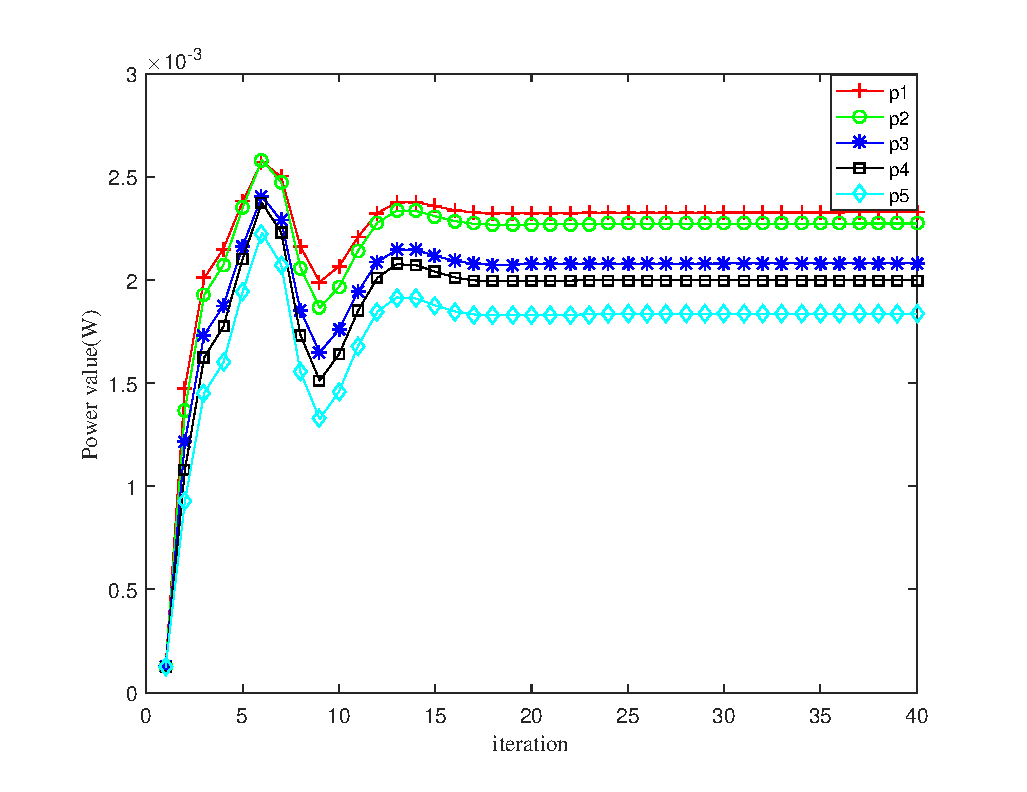
\includegraphics[width=7cm]{figures//pp.eps}
\caption{Power convergence performance.}
\label{F2}
\end{figure}

\begin{figure}[H]
\centering
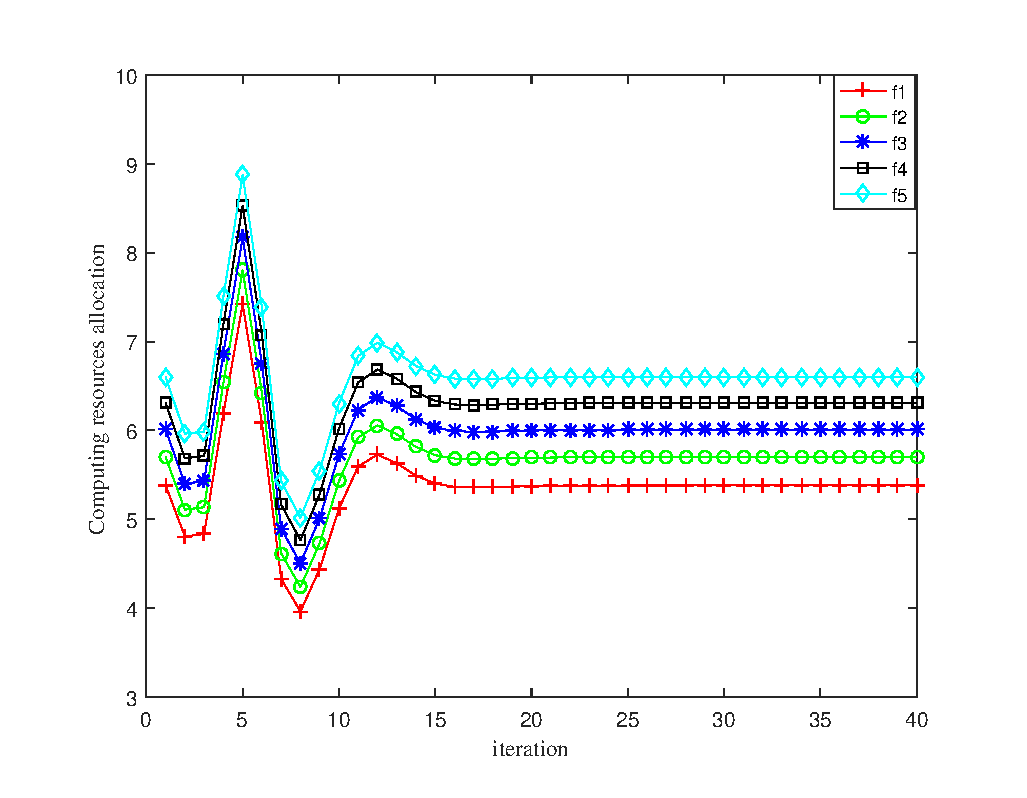
\includegraphics[width=7cm]{figures//ff.eps}
\caption{computing resource which cloud allocation to RSU.}
\label{F3}
\end{figure}

\begin{figure}[H]
\centering
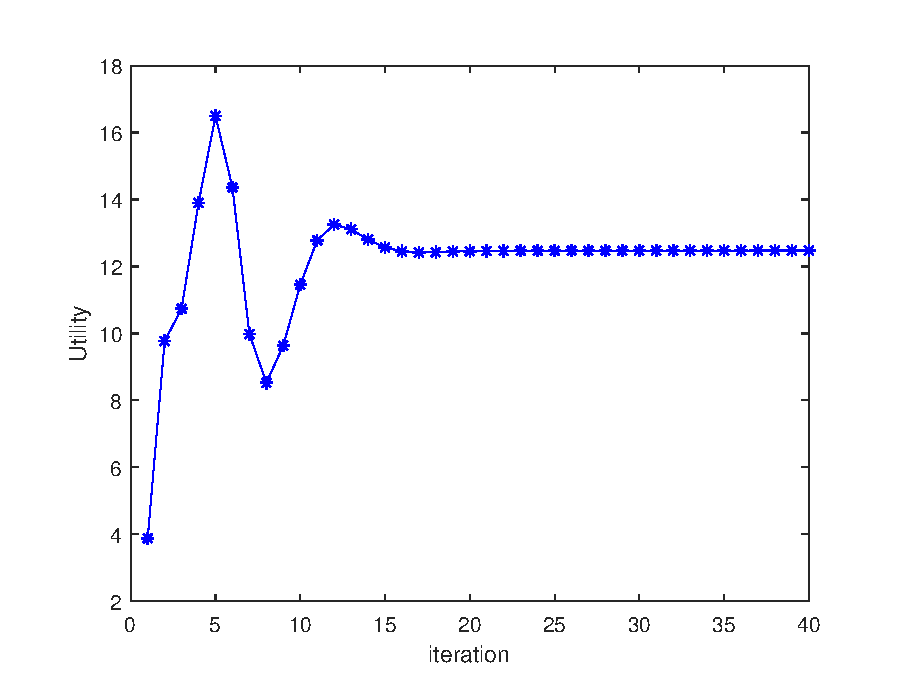
\includegraphics[width=7cm]{figures//ee.eps}
\caption{Convergence of average system utility.}
\label{F4}
\end{figure}

Fig. \ref{F2} and Fig. \ref{F3} show the power allocation of each vehicle transmitter and the corresponding computing resource which cloud allocation to RSU in Algorithm~\ref{alg:algorithm1}, respectively. It can be seen that the computing resources allocated in the cloud peak at the fifth iteration and begin to decline because of the limitation of total computing resources $f_{total}$ from the cloud. The corresponding power resource allocation also changes due to computing resources allocation under robust power control and task offloading scheduling.

Fig. \ref{F4} shows the convergence of the total utility of the system under joint optimization, and it can be seen that the convergence trend of the total utility of the network system is related to power allocation and computing resource allocation, this phenomenon is reasonable due to the definition of $U$ in \eqref{E12}. $R_i$ increases logarithmically as the power vector $\mathbf{p}$ increases, the upload time $t_{i,up}$, as the denominator of $U$, will decrease with the increase of power vector $\mathbf{p}$ and as the executive utility of the numerator part, $t_{i,exe}$ decreases inversely proportional with the increase of computing power vector $\mathbf{f}$, causing the numerator to increase with the increase of vector $\mathbf{f}$.

In the MEC-Enabled vehicular cloud system. It is unrealistic not to take into account the mobility of the vehicle, we then investigated the impact of vehicle mobility on system performance. Assume the variation of the vehicles�� speed is negligible within the reference time interval. In order to further illustrate the influence of speed-induced Doppler shift on system performance, the comparison experiment between the benchmark value and the increasing speed measurement under the condition of constant vehicle speed is simulated in the system.

Since the relative speed in the V2R link is zero, And the speed of all vehicles is the same in the same network there is no Doppler effect. Then the vehicle speed on the road is set to 20 m/s, 30 m/s, 40 m/s, 50 m/s and 60 m/s, respectively��It can be seen from Fig. \ref{F5} that with the increase of vehicle speed, the utility value of the vehicular network decreases, This is because the higher speed will cause a greater Doppler frequency shift in the network, increase channel uncertainty. The result also proves that methods tend to obtain better utility when the vehicle speed is low.
\begin{figure}[H]
\centering
\includegraphics[width=8cm]{figures//diffspeed.eps}
\caption{Comparison of average system utility against different speed.}
\label{F5}
\end{figure}

In order to further verify the performance of the proposed scheme after considering the mobility of the vehicle, the Fig. \ref{F6} describes the effect of the same speed and different speeds of each vehicle under different $\varepsilon_1$ on the total utility, and it can be seen from the figure that with the change of $\varepsilon_1$, the system utility also changes, and the utility at different speeds of each vehicle is higher than that of all vehicles at the same speed, which characterizes the high robustness of the proposed method in complex dynamic vehicle networks.
\begin{figure}[H]
\centering
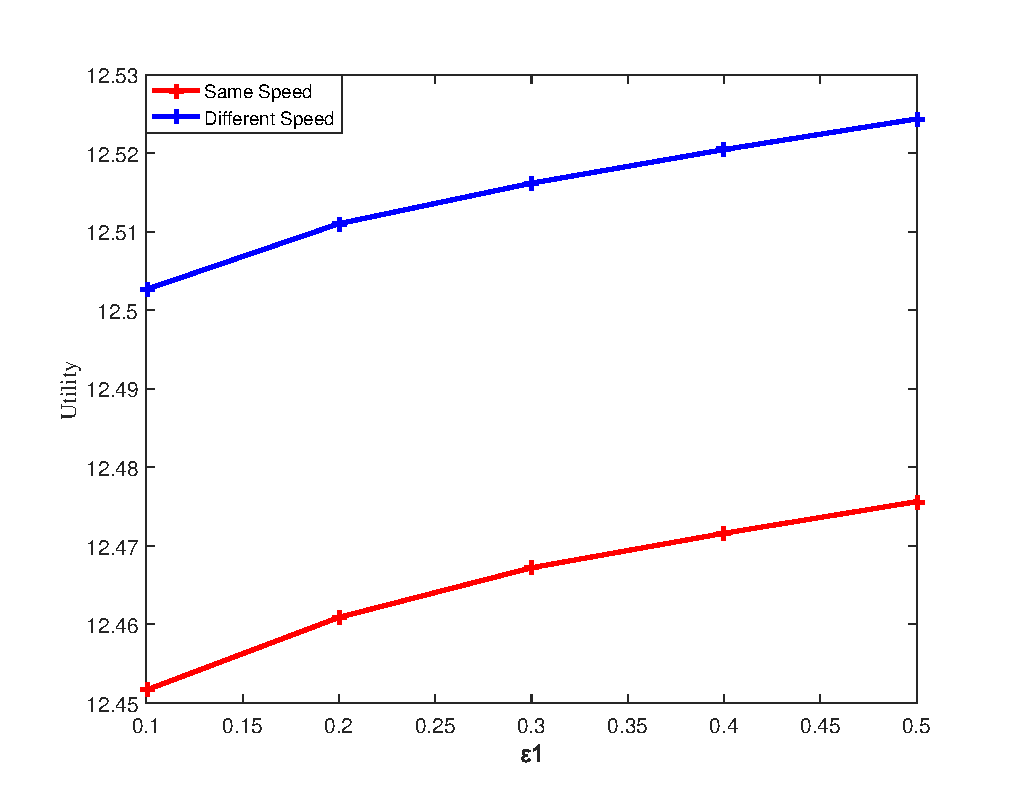
\includegraphics[width=8cm]{figures//diff_e1.eps}
\caption{Comparison of average system utility against different $\varepsilon_1$.}
\label{F6}
\end{figure}

In terms of computing resources allocation, we choose the default task input size as $ d_u=420KB$ (following \cite{Xu2015}), We now evaluate the system utility performance against different benchmark schemes. The purpose of this section is to show the convergence of our proposed algorithm and its performance is better than three benchmark schemes through some simulation results. The benchmark schemes are described as follow
\begin{itemize}
\item[1)]``Independent Offloading and power control'' (denoted as ``IOP''), the vehicles independently make power control and the computing resources allocation.
\item[2)]``��Without vehicle power control''(denoted as ``Without-VPC''), the transmit power of the vehicles is set as average power during the offloading.
\item[3)]``��Without computing resources allocation'' (denoted as ``Without-CRA''), the transmit power of the vehicles is set as average power during the offloading.
    %Similar to [?]Jiang2016  Similar to: \cite{Jiang2016},
\end{itemize}
Fig. \ref{F7} is the iterative convergence of the total utility of the system in different cases, and it can be seen from the figure that the robust joint optimization performance is better than the other three cases. It can be seen that with the increase of the number of iterations, the four methods converge to a stable value, among which the performance of proposed scheme is the best.
\begin{figure}[H]
\centering
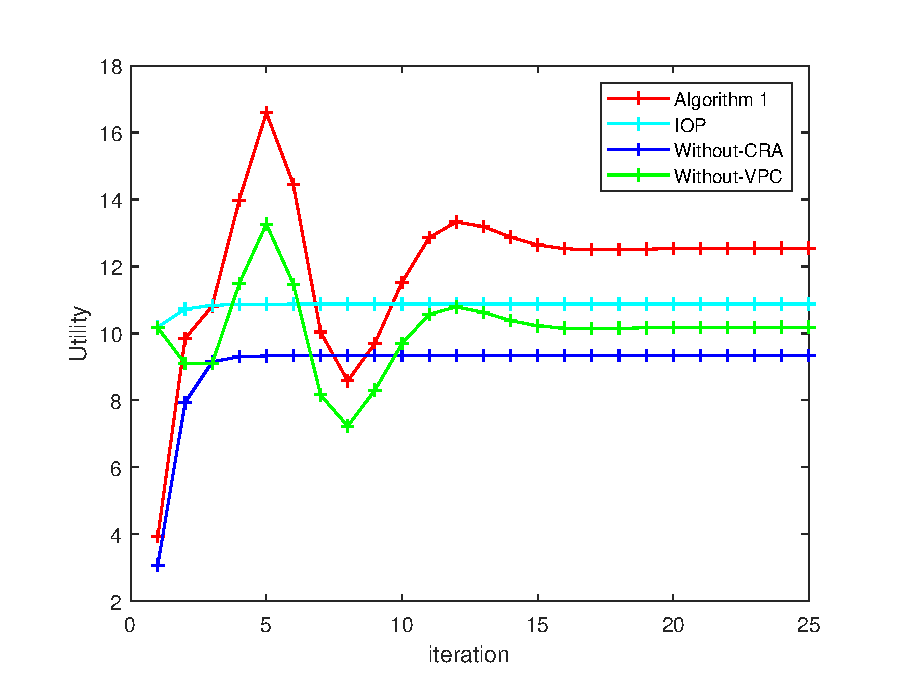
\includegraphics[width=8cm]{figures//compare.eps}
\caption{System utility convergence under different methods.}
\label{F7}
\end{figure}
In order to reflect a more realistic situation, the CPU task lode (Megzcycles) required for each vehicle are often different, so we set the CPU task load (Megzcycles) of the five vehicles to 1600, 1700, 1800, 1900, 2000.

As we can see, with the increase of the ratio of iteration, the average system utility of vehicles changes gradually and tends to be stable. In the independent optimization process, the computing resource allocation is carried out first, and the optimal power allocation is not known at this time, and the power and computing resource alternate optimization method is used, and the corresponding optimal value can be obtained for each iteration. Individual optimization is to first optimize the power vector $\mathbf{p}$, and after obtaining the result, the result is used for the optimization of computing resources, and then the computing resources are optimized, and finally, the utility of the system is obtained. However, if joint optimization is used, then both variables can get the optimal value.
\begin{figure}[H]
\centering
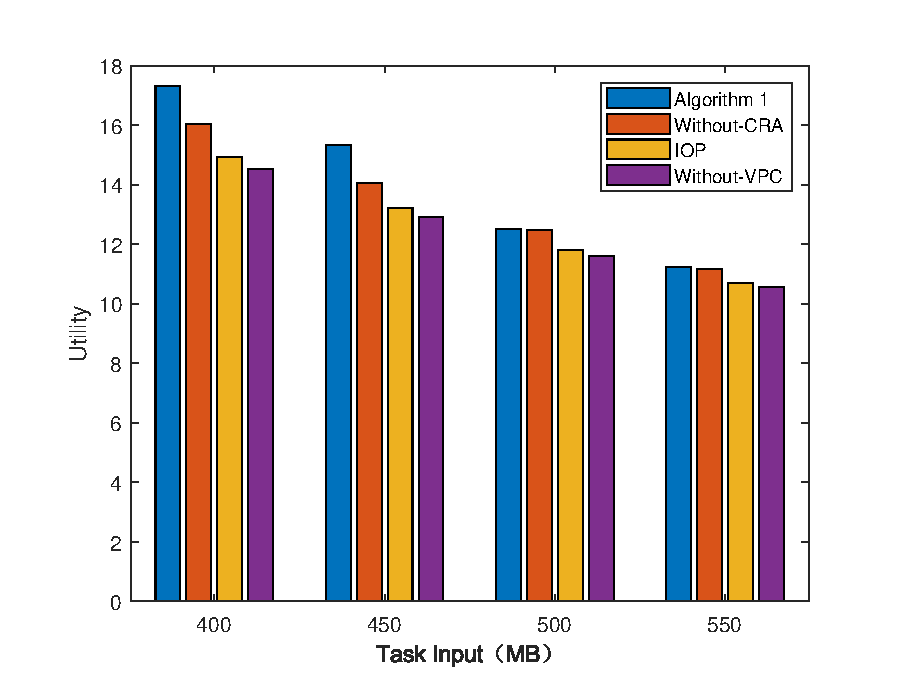
\includegraphics[width=8cm]{figures//diff_dup.eps}
\caption{Comparison of average system utility against different task input size $d_u$.}
\label{F8}
\end{figure}
\begin{figure}[H]
\centering
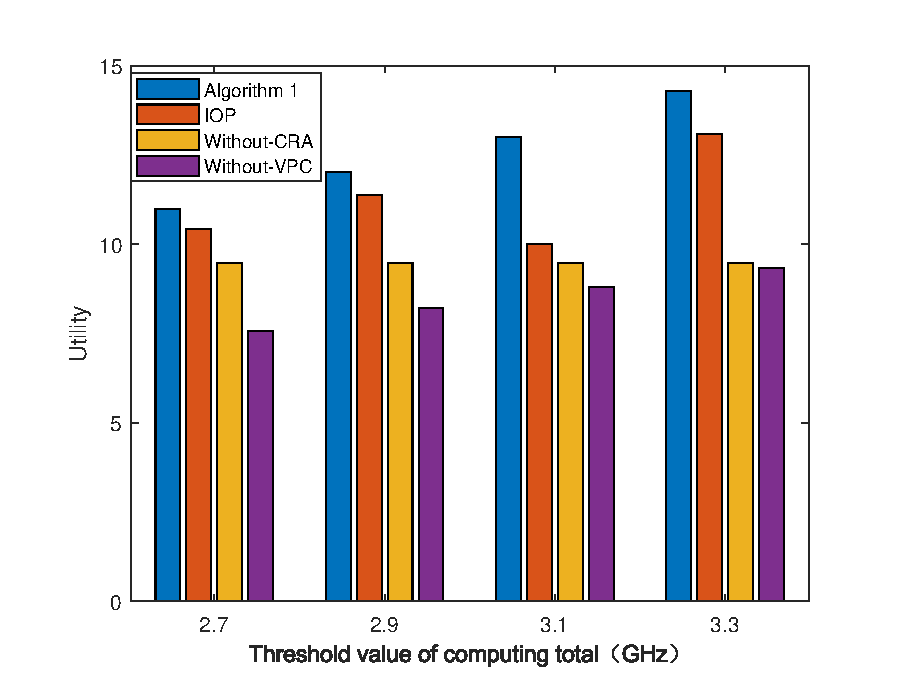
\includegraphics[width=8cm]{figures//diff_total.eps}
\caption{Comparison of average system utility against different $f_{total}$.}
\label{F9}
\end{figure}
\begin{figure}[H]
\centering
\includegraphics[width=8cm]{figures//diff_c.eps}
\caption{Comparison of average system utility against different task workloads $c_{i,e}$.}
\label{F10}
\end{figure}
The average system utility of the four competing schemes are plotted in Fig. \ref{F8} with different values of $d_u$. It can be seen that the average system utilities of all schemes decrease with the task input size. Moreover, we observe that the performance gains of the proposed scheme over the other schemes also follow the similar trend.
The total system cost comparisons with different $f_{total}$ are shown in Fig. \ref{F9}, due to the limited computation capability at the cloud, when the computation capability is small, the system utility tend to small.
We can clearly see that as the data size increases, the system utility tend to small in Fig. \ref{F10}. This is because when the tasks require more upload time with more data size.
\section{Conclusions}\label{Conclusions}
This paper focuses on the Power Control and Task Offloading for Cloud Assisted MEC in Vehicular Networks with channel uncertainty and co-channel interference. The optimization scheme attempt to guarantees vehicles�� QoS when there exists a maximized utility requirement. Due to the existence of channel uncertainty, the probability forms of interference, delay, and delivery rate constraints are performed. The underlying optimization problem was formulated as a joint robust power control and task offloading scheduling program, which is very difficult to solve to optimal, then the SCA technique is applied to transform the non-convex problem of variables coupling into a treatable convex problem. The task offloading and power allocation algorithm is developed to achieve practical execution scheme. Simulation results showed that our heuristic algorithm performs closely to the optimal solution and significantly improves the average system offloading utility over traditional approaches.
\bibliography{reference}
\bibliographystyle{IEEEtran}
%\bibliographystyle{plainnat}
%\bibliographystyle{unsrtnat}
\end{document}
